\documentclass[9pt, twocolumn, twoside, lineno]{pnas-new}
% Use the lineno option to display guide line numbers if required.

% PNAS研究论文模板
\templatetype{pnasresearcharticle} % Choose template 
% {pnasresearcharticle} = Template for a two-column research article
% {pnasmathematics} %= Template for a one-column mathematics article
% {pnasinvited} %= Template for a PNAS invited submission
	
% 文章标题:“流域尺度的水资源利用体系:过渡框架和发展困局”
\title{Water resource utilization regimes at a basin scale: transition framework and development traps}

% Use letters for affiliations, numbers to show equal authorship (if applicable) and to indicate the corresponding author
% 作者列表
\author[a, b]{Shuang Song}  % 宋爽,一作
\author[a, b, 1]{Shuai Wang}  % 王老师,通讯
\author[a, b]{Bojie Fu}  % 傅老师
\author[c, d]{Xutong Wu}  % 武旭同

% 机构列表
\affil[a]{ % 北师大地表国重
	State Key Laboratory of Earth Surface Processes and Resource Ecology, 
	Faculty of Geographical Science, 
	Beijing Normal University, 
	Beijing 100875, 
	P.R. China
}
\affil[b]{ % 北师大地理学部
	Institute of Land Surface System and Sustainability, 
	Faculty of Geographical Science, 
	Beijing Normal University, 
	Beijing 100875, 
	P.R. China
}
\affil[c]{ % 北大城环
	College of Urban and Environmental Sciences, 
	Peking University, 
	Beijing 100871, 
	P.R. China
}
\affil[d]{ % 中科院生态中心
	State Key Laboratory of Urban and Regional Ecology, 
	Research Center for Eco-Environmental Sciences, 
	Chinese Academy of Sciences, 
	Beijing 100085, 
	P.R. China 
}

% Please give the surname of the lead author for the running footer
% 领衔作者
\leadauthor{Song} 

% Please add a significance statement to explain the relevance of your work
% PNAS特有的“Significance陈述”,用不超过120个字来说明研究的意义和亮点
\significancestatement{Authors must submit a 120-word maximum statement about the significance of their research paper written at a level understandable to an undergraduate educated scientist outside their field of speciality. The primary goal of the significance statement is to explain the relevance of the work in broad context to a broad readership. The significance statement appears in the paper itself and is required for all research papers.}

% Please include corresponding author, author contribution and author declaration information
\authorcontributions{ % 作者的相应贡献
	Shuai Wang and Bojie Fu designed this research,
	Shuang Song performed the research and analysed data,
	Shuang Song, Xutong Wu wrote the paper.
}
\authordeclaration{ % 利益冲突陈述
	The authors declare no competing interests.
}

% 如果有共同一作的情况,则uncomment下面这行代码的注释
%\equalauthors{\textsuperscript{1}A.O.(Author One) contributed equally to this work with A.T. (Author Two) (remove if not applicable).}

% 通讯作者信息
\correspondingauthor{\textsuperscript{1}To whom correspondence should be addressed. E-mail: shuaiwang@bnu.edu.cn}

% 关键词,三到五个
% At least three keywords are required at submission. Please provide three to five keywords, separated by the pipe symbol.
\keywords{Water resource management  $|$ Human-water relationship $|$ Water scarcity $|$ Sustainable development} 

%tag 摘要
\begin{abstract}
	% 水资源(water resources)对人类社会的重要性,人类对水资源的影响,
	The importance of water resources to human society, 
	the impact of humans on water resources, the relationship between humans and... 
	% 人类与水资源之间逐渐建立了复杂的{人水关系(human-water relationship)},并形成了{"水资源利用体系 (water utilization regime)"}。
	A complex human-water relationship is gradually being established between water resources.
	And resulted in water utilization regime.
	%通过在流域尺度分析(analyse)水资源利用体系来刻画(depict)人水关系,有助于识别(distinguish)和理解(understand)流域发展过程中面对的困局(traps),
	% 进而为流域{综合水资源管理 Integrated water resources management}和{协调发展(develop in a coordinated way}提供理论依据。
	This helps to identify and understand the traps in the development of river basins, 
	thus providing a theoretical basis for integrated water resources management and development in a coordinated way.
	
%这里,同时考虑了流域水资源利用的{“资源压力(stress)”},{“倾向性(lopsidedness)”}和{“格局(pattern)”},
% 我们提出了{流域协调发展指数 (Basin coordinated development index)},用以归纳(summarise)流域水资源利用体系的发展变化情况。

% 以黄河(世界上人为干预最严重的大河之一)为例,流域协调发展系数的变化结果指示,流域的水资源利用体系自上世纪50年代起先后历经了三个不同的阶段。

% 其中1977年前后经历的第一次体系转变(regime shift)主要表现为水资源利用压力的迅速增加,
% 而1993年前后历经的第二次体系转变则主要由水资源利用的倾向性和格局来驱动。

% 这表明黄河流域发展过程中曾一度陷入资源困局,而后成功通过积极调整水资源利用体系摆脱了困局,但当前仍面临陷入结构困局的风险。
% 最后,结合相关理论,我们进一步总结了流域水资源利用体系的一般过渡框架(transition framework),
% 该框架对理解水资源利用体系的变化及发展过程中面临的相关困局具有指导意义。
\end{abstract}


\dates{This manuscript was compiled on \today}
\doi{\url{www.pnas.org/cgi/doi/10.1073/pnas.XXXXXXXXXX}}


\begin{document}

\maketitle
\thispagestyle{firststyle}
\ifthenelse{\boolean{shortarticle}}{\ifthenelse{\boolean{singlecolumn}}{\abscontentformatted}{\abscontent}}{}

% If your first paragraph (i.e. with the \dropcap) contains a list environment (quote, quotation, theorem, definition, enumerate, itemize...), the line after the list may have some extra indentation. If this is the case, add \parshape=0 to the end of the list environment.

% tag 引言第一段
% 水资源在人类世的重要性,是支持人类社会发展的基础
\dropcap{W}ater, at “the centre of the planetary drama of the Anthropocene”, 
is not only essential for myriad Earth system processes,
but also a key resource supporting development of human societies in various aspects \cite{gleesonIlluminatingWaterCycle2020}.
% 但同时, 人类的改造也深刻影响了自然水循环过程, 相关变化可能影响人水系统功能的不利转变,并带来发展困局。
At the same time, however, human's modification has profoundly influenced water processes 
and related changes may lead to adverse transitions in functions of human-water systems,
along with various development traps. 
% 世界上诸多大河流域都是经济和文明发展的中心,同时也是面临人类世压力挑战的主要地区,亟需综合水资源治理以实现可持续发展
Facing major challenges of the Anthropocene, many of the world's big river basins are also centres of economy and civilization 
and urgently in need for integrated water resources management toward sustainability. \cite{bestAnthropogenicStressesWorld2019}
% 因此理解人类社会发展与水资源利用的复杂关系,对此有帮助
Therefore, understanding the complex relationship between human societies and water resources utilization 
provides underlying supports to development in a coordinated way, at a basin scale.



% tag 引言第二段
% Regime的定义。
Regime is a general term of system’s structure and function 
and one of the most explanatory perspectives when analysis interactions within a coupling system, 
like human and water.
% Regime的转变
Since widespread fluctuating disturbances in social development and natural water resources were out of consideration, 
water utilization regime only will be driven shifting when reorganizations occurred and the tipping points reached.
% Regime过渡性的存在。
As many large river basins had all experienced phases of accelerated water exploitation, over-exploitation of water resource,
and integrated water management, it is a reasonable assumption that existence of a transitional water utilization regime 
corresponds to development of societies. 
% 过渡性有助于理解流域存在的问题
Understanding the transitional nature of water resource regimes, therefore, can help to diagnosis and predict development traps, 
which is crucial for integrated management and coordinated development at a basin scale regard to sustainability.
% 对过渡性的研究还很少
% Despite pervasive and important, there is lacking of formal framework to interpret the water utilization regimes, 
% with much fewer attempts in developing effective methods to detect them and their transitions as well. 
Despite pervasive and important as it is, there is lacking of effective method to detect the water utilization regimes and their shifts, 
with much fewer attempts to develop formal models of its transitions as well. 



% Tag 引言第三段
% 作为是古老而常青的现象,前人已经从不同视角刻画了人水关系.
The key to analysis water utilization regimes is to understand the interactions between human societies and water resources, 
which have been depicted from different dimensions, as an ancient but evergreen topic.
% 首先,因为水资源的稀缺性和全球用水量的增加,受到最广泛关注的是人类社会面临的水资源压力。
Firstly, the most widespread concern is the rising stresses on human societies with regard to water resources.
% 人类取水量增加,不灵活部分增长,尽管社会通过不断发展拥有更强大的调蓄能力,但世界上绝大多数流域都面临着更大的水资源压力。
Even though the stocks of water in increasing artificial reservoirs are helpful to water resources availability, 
highly stressed basins still characterized by high water consumption intensities and a major constraint to socio-economic development,
driven by a significant increase in water extractions and a larger share of inflexible water utilization during the last century.
\cite{postelHumanAppropriationRenewable1996, greveGlobalAssessmentWater2018a, qinFlexibilityIntensityGlobal2019}
% 其次,随着工业迅猛发展和生态建设的需要,社会对水资源的利用的倾向性也发生了转变。
Secondly, as the need of industrial and ecological developments, tendentiousness of water utilization changed with.
% 尽管主要的用水方式还是农业灌溉,但工业的经济和用水都正在增长,且存在潜在的冲突。
Despite a major water utilization of agricultural irrigation dominating most of the river basins,
there are significant growths and preferential tendentiousness in the economy profits and water consumption regarding industry, 
leading a high potential for conflict between the industrial and agricultural sectors.
\cite{liuWaterScarcityAssessments2017, florkeWaterCompetitionCities2018}
% 最后,由于水的可用性本质上是区域问题,水资源利用的格局也很重要
Thirdly, since water availability and utilization are inherently regional concerns, patterns of also play an important role.
% 全球总的取水量很少,但缺水地区很多
Although only 10\% of available water is withdrawn on global average, about 30\% of population live in highly water-stressed areas,
where dominated sections regarding water utilization are various. 
\cite{wadaWedgeApproachWater2014, okiGlobalHydrologicalCycles2006}
% 此外,人类活动还在改变这一格局
In addition, human activities are still changing this pattern, 
since positive impacts caused by human interventions mostly occur in upper regions 
whereas aggravated water resources downstream, in many basins around the world.
\cite{veldkampWaterScarcityHotspots2017}
% 将三种视角结合,就是“水资源利用体系”。
Although existing researches have evaluated the aspects of water resource utilization from these different dimensions, 
we still cannot obtain a coherent understanding of regime regard to social development and water utilization, without integrating them.


% tag 讨论最后一段
% 这里我们整合了三个方向,提出了描绘流域人水关系的指数
Here, by integrating three above mentioned dimensions of water utilization, 
we develop an Integrated Water Resources Utilization (IWRU) Index at a basin scale
to give a sketch of relationships between human societies and their water utilization.
% 使用案例研究
Then, by applying this index to the Yellow River Basin, China,
we analysed water utilization regimes and their shifts in this typical basin of anthropogenic impacts, 
with change points detection and contribution decomposition methods following.
% 指出发展困局
In addition, combining model and data analysis, 
we further identify resource and development traps that have been exposed by regimes' shifting.
% 最后总结出一般性框架
Finally, refer to the existing theories, we summarized a general transition framework of water utilization regimes, 
which can be a useful guideline for basins to predict development traps and to develop in a coordinated way.


\section*{Results}
%tag 结果1: 指数划分结构
\subsection*{Water utilization regimes}
% 这一节主要展示BCDI的变化趋势和WUR的划分
By the two significantly detected change points,
the changes of IWRU index are split into three periods, 
whose slopes are various and mainly contributed by different factors \ref{fig:IWRU}.
\begin{figure}%[htbp]
	\centering
	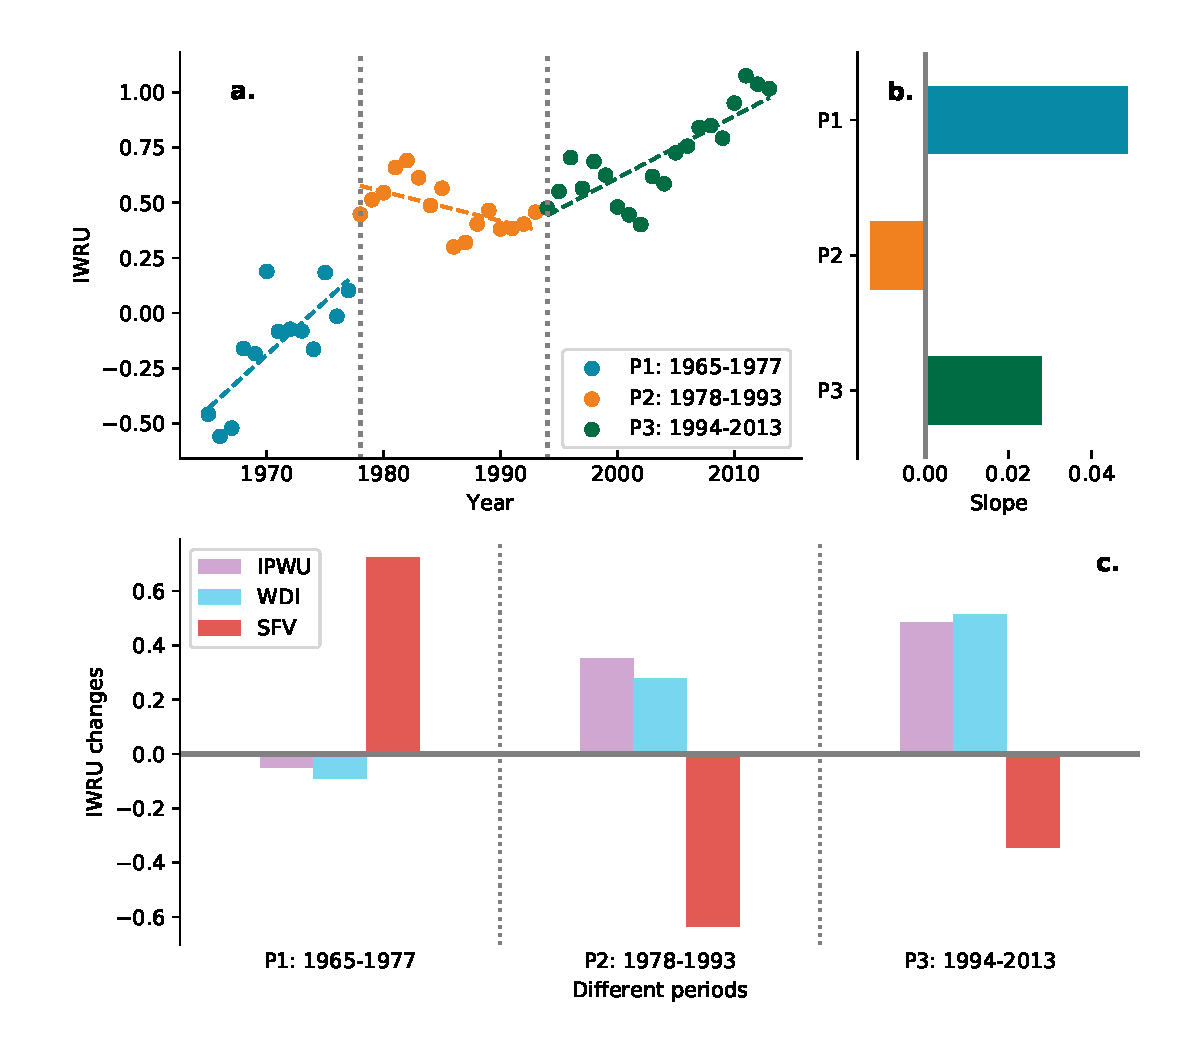
\includegraphics[width=\linewidth]{../../figures/main_text/index}
	\caption{Changes of the IWRU index. 
	\textbf{A,} with two change points in 1978 and 1994, three periods were detected in trend of the IWRU.
	\textbf{B,} changes of IWRU in three periods have various slopes, while the second period have a negative growths rate.
	\textbf{C,} changes of the IWRU within three certain periods, which have different main contributors.
	}
	\label{fig:IWRU}
\end{figure}
% 接下来分句介绍每个阶段的特征
% 第一阶段
In the first period (P1, 1965-1978), the IWRU index had a rapidly increasing 
and the lightening of water stresses made the most striking contribution (xx\%), 
while tendentiousness and pattern of the water utilization had slight negative contribution.
% 第二阶段
In the second period (P2, 1979-1994), the IWRU index experienced a slight drop, 
despite positive contributions of tendentiousness and pattern of water utilization,
because of increasing stresses on water resource playing a larger negative role (xx\%). 
% 第三阶段
However, as the further increasing of positive contributions of water utilization tendentiousness and pattern, 
and decelerations of water stresses in the third period (P3, 1995-2013), a positive growth of the IWRU returned.
% 总的来说,用水三个维度的组合呈现出阶段特征明显,但缓慢过渡的变化趋势
Taken together, combining the three dimensions of water resources utilization, 
whose regimes have clear phase-characteristics with gradual transitions between different phases}.

%tag 结果2
\subsection*{Changes between different regimes}

\begin{figure}%[htbp]
	\centering
	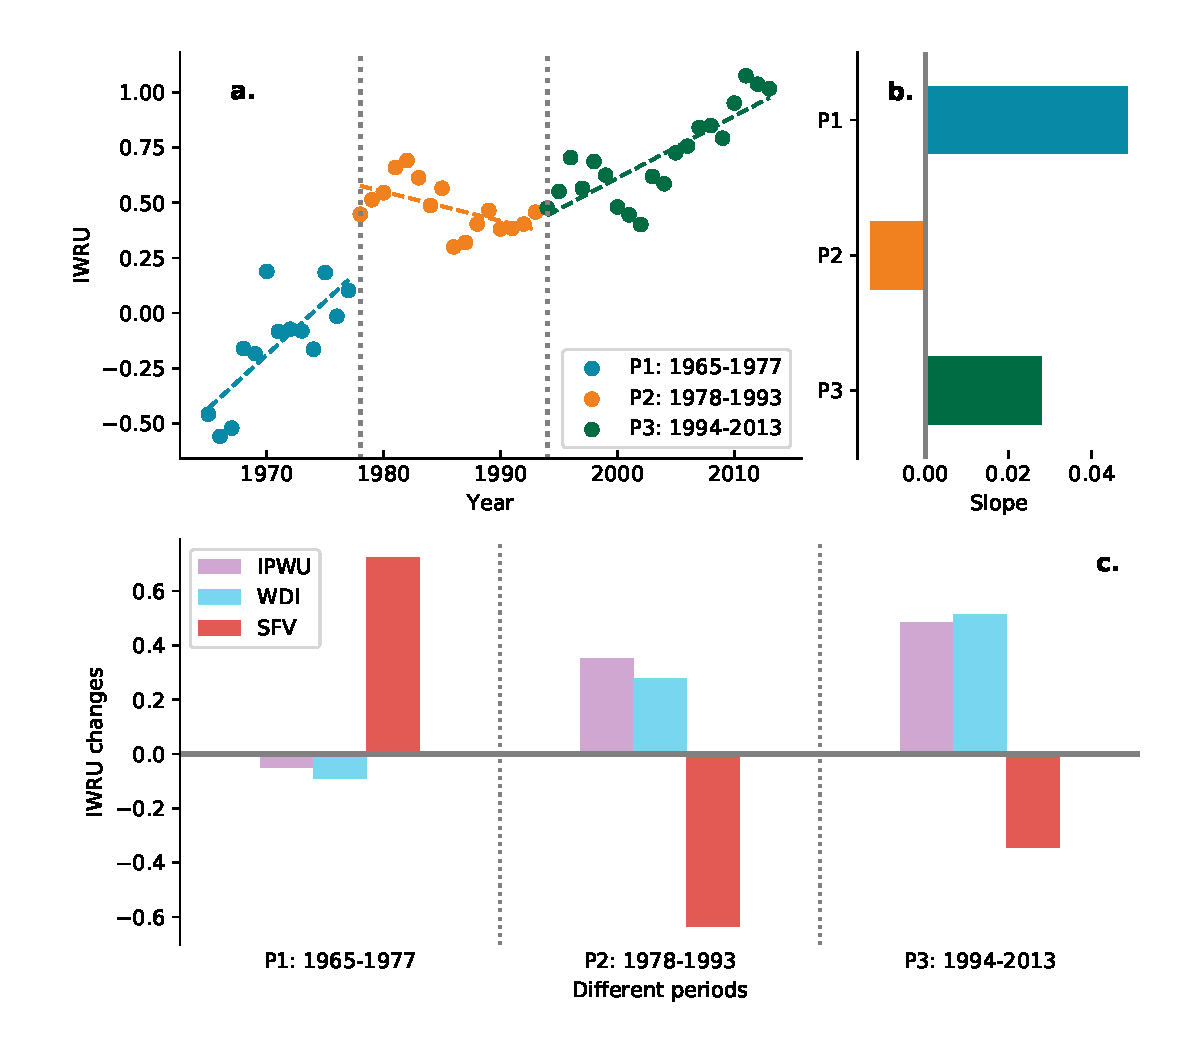
\includegraphics[width=\linewidth]{../../figures/main_text/index}
	\caption{Placeholder image of a frog with a long example legend to show justification setting.}
	\label{fig:changes}
\end{figure}

\subsection*{Main drivers of the regime shifts}

\subsection*{Language-Editing Services}
Prior to submission, authors who believe their manuscripts would benefit from professional editing are encouraged to use a language-editing service (see list at www.pnas.org/page/authors/language-editing). PNAS does not take responsibility for or endorse these services, and their use has no bearing on acceptance of a manuscript for publication. 


\subsection*{Digital Figures}

EPS, high-resolution PDF, and PowerPoint are preferred formats for figures that will be used in the main manuscript. Authors may submit PRC or U3D files for 3D images; these must be accompanied by 2D representations in TIFF, EPS, or high-resolution PDF format. Colour images must be in RGB (red, green, blue) mode. Include the font files for any text.

Images must be provided at final size, preferably 1 column width (8.7 cm). Figures wider than 1 column should be sized to 11.4 cm or 17.8 cm wide. Numbers, letters, and symbols should be no smaller than 6 points (2 mm) and no larger than 12 points (6 mm) after reduction and must be consistent. 

Figures and tables should be labelled and referenced in the standard way using the \verb|\label{}| and \verb|\ref{}| commands.


\subsection*{Tables}
Tables should be included in the main manuscript file and should not be uploaded separately.


\begin{table}%[htbp]
	\centering
	\caption{Comparison of the fitted potential energy surfaces and ab initio benchmark electronic energy calculations}
	\begin{tabular}{lrrr}
		Species & CBS & CV & G3 \\
		\midrule
		1. Acetaldehyde & 0.0 & 0.0 & 0.0 \\
		2. Vinyl alcohol & 9.1 & 9.6 & 13.5 \\
		3. Hydroxyethylidene & 50.8 & 51.2 & 54.0\\
		\bottomrule
	\end{tabular}
	
	\addtabletext{nomenclature for the TSs refers to the numbered species in the table.}
\end{table}

% tag 讨论
\section*{Discussion}

\subsection*{Transition Framework}
Tables should be included in the main manuscript file and should not be uploaded separately.

\begin{figure}%[htbp]
	\centering
	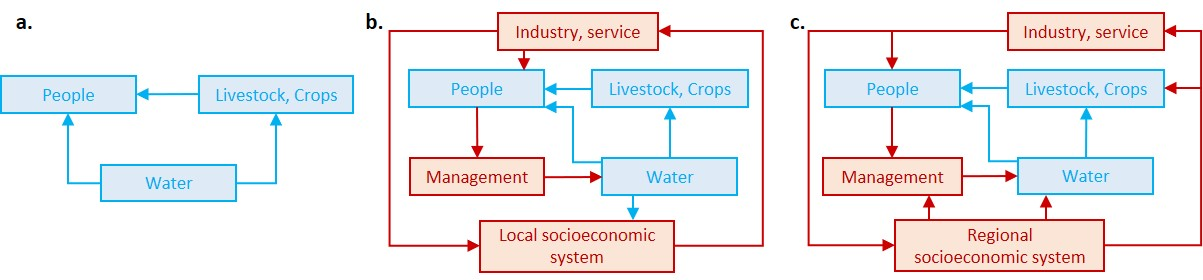
\includegraphics[width=\linewidth]{../../figures/main_text/framework}
	\caption{Placeholder image of a frog with a long example legend to show justification setting.}
	\label{fig:framework}
\end{figure}

\subsection*{Development Traps}

%tag 研究方法
\matmethods{Please describe your materials and methods here. This can be more than one paragraph, and may contain subsections and equations as required. Authors should include a statement in the methods section describing how readers will be able to access the data in the paper. 
	
	\subsection*{Water utilization regime index}
	Example text for subsection.
	\subsubsection*{Stresses}
% 提出了很多的指标度量水压力,如水资源压力指数,水资源xxx等
	Various metrics, therefore, proposed for water stress 
	(e.g. water scarcity, water stresses index, scarcity-flexibility-variability index), 
	where the dimensions of human impact are increasingly valued.
	% 其中SFV指数比较有用
	Among of them, by taking changes of water flexibility and variability into account, 
	the scarcity-flexibility-variability (SFV) index focus more on dynamic responses to water resources in developing perspective,
	which considered a valid indicator of temporal changes in water stresses.
	\subsubsection*{Lopsidedness}
	% xxx等人通过考虑消费品中的水消耗提出了虚拟水理论
	% 但随着水资源利用方式的变迁,在其基础上兴起的水足迹研究,则进一步泛化了水相关的产品和服务概念。
	% 如今,世界非产品形式供给于人类的水资源已达xx%,范围包含了xxxxxx等方式,人类在“消耗水”向“利用水”和的倾斜。

	\subsubsection*{Patterns}

	\subsection*{Change points detection}
	
	\subsection*{Contribution decomposition}
}

\showmatmethods{} % Display the Materials and Methods section

\acknow{Please include your acknowledgments here, set in a single paragraph. Please do not include any acknowledgments in the Supporting Information, or anywhere else in the manuscript.}

\showacknow{} % Display the acknowledgments section

% Bibliography
\bibliography{my-papers}
	
\end{document}